\documentclass[]{article}
\usepackage{listings}
\usepackage{graphicx}
\usepackage{xcolor}
\usepackage{mathtools}
\usepackage[T1]{fontenc}
\usepackage[margin=1in, top=1in, bottom=1in]{geometry}
\definecolor{lightGray}{HTML}{ECECEC}
\lstset{language=python}
\lstset{basicstyle=\footnotesize\ttfamily, tabsize=4, breaklines=true}
\lstset{backgroundcolor = \color{lightGray}, framexleftmargin=10pt, framexrightmargin=10pt}
\graphicspath{{./pictures/}}

%opening
\title{Računalna animacija - 3. laboratorijska vježba}
\author{Ana Bagić, 0036515780}

\begin{document}

\maketitle
\section{Pokretanje}

Nakon kloniranja repozitorija lokalno na uređaj, može se pokrenuti projekt. Zbog korištenja Maven-a i biblioteke OpenGL nisam uspjela pronaći jednostavno rješenje koje bi pokrenulo projekt iz komandne linije zbog više jar datoteka. Međutim, importanjem projekta \textit{lab03} u neko razvojno okruženje (npr. IntelliJ koji sam koristila), jednostavno je pokrenuti aplikaciju. Potrebno je postaviti konfiguraciju, kako se vidi na slici \ref{fig:config} (bitno je da je verzija Jave 11).
\begin{figure}[h]
	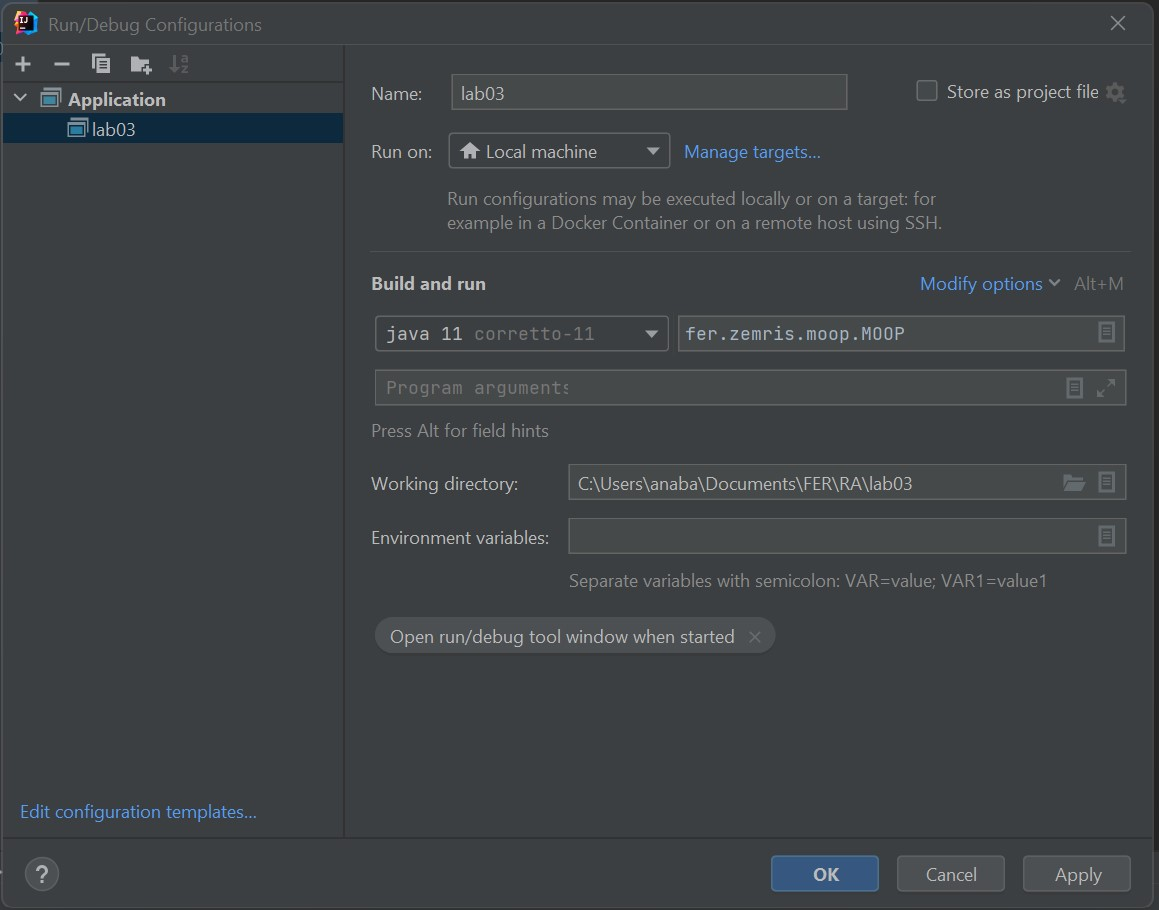
\includegraphics[scale=0.7]{config.jpg}
	\centering
	\caption{Konfiguracija za pokretanje}
	\label{fig:config}
\end{figure}
\pagebreak

\section{Opis rada}
U ovom radu implementirala sam grafički prikaz algoritma višekriterijske optimizacije NSGA-II u Javi koristeći OpenGL (JOGL) biblioteku. Točnije, radi se o vizualizaciji samo dvokriterijske optimizacije zbog ograničenja s prikazom više dimenzija.

\subsection{NSGA-II algoritam}
NSGA-II (\textit{Non-dominated Sorting Genetic Algorithm II}) algoritam je jedan od najpoznatijih algoritama trenutno korištenih za višekriterijsku optimizaciju. Nastao je kao poboljšanje algoritma NSGA, tako da uvodi elitizam, koristi nedominirano sortiranje i mjeru \textit{crowding distance}. Glavna ideja algoritma je sortirati populaciju rješenja u različite fronte, po tome koliko su rješenja "dobra", odnosno po kriteriju nedominacije.\\

Svojstvo nedominacije znači da neko rješenje barem po nekom kriteriju bolje od ostalih koja nisu u toj fronti, odnosno da nije dominirano ostalim rješenjima. Po tom svojstvu rješenja se slažu u fronte, gdje je prva fronta ona koja sadrži rješenja s najvećom dobrotom, druga ona malo lošija i tako dalje. Pseudokod algoritma može se vidjeti na slici \ref{fig:nsgaii} preuzete iz prezentacije o višekriterijskoj optimizaciji iz kolegija \textit{Optimiranje evolucijskim računanjem}.

\begin{figure}[h]
	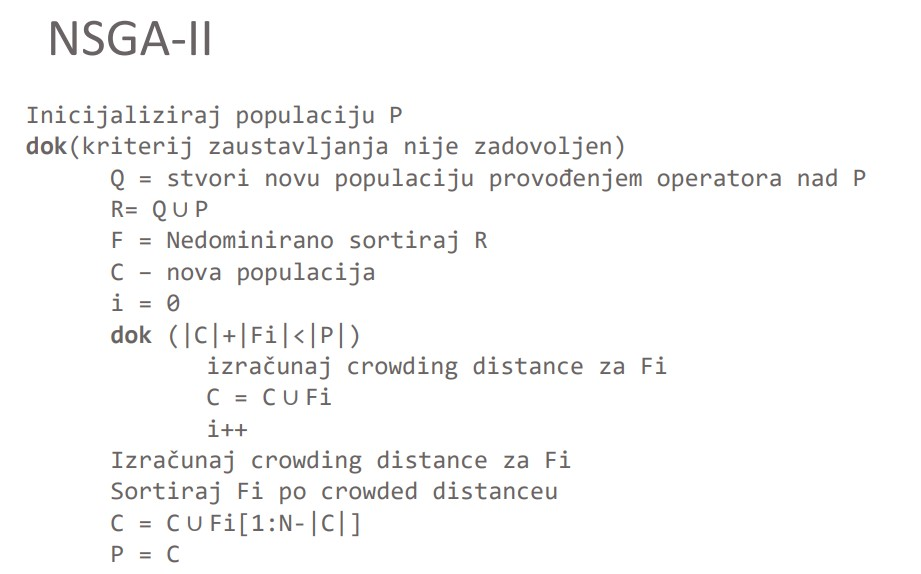
\includegraphics[scale=0.8]{nsgaii.jpg}
	\centering
	\caption{Pseudokod algoritma NSGA-II}
	\label{fig:nsgaii}
\end{figure}

\textit{Crowding distance}, odnosno "udaljenost gužve" govori nam koliko su blizu susjedna rješenja iz te fronte. Korištenjem te mjere, daje se prednost rješenjima koja sadrže manje ostalih rješenja iz iste fronte u blizini. Time se održava raznolikost rješenja.
\pagebreak

\subsection{Vizualizacija}

U ovom primjeru koristila sam sljedeći problem. Minimiziraj funkcije:
\begin{equation}
	f(x, y) = x
\end{equation}
\begin{equation}
	g(x, y) = \frac{1 + y}{x}
\end{equation}

uz ograničenja:
\begin{equation}
	0.1 <= x <= 1
\end{equation}
\begin{equation}
	0 <= y <= 5
\end{equation}

Odmah prilikom pokretanja aplikacije, prozor izgleda kao na slici \ref{fig:before}. Algoritam se može pokrenuti pritiskom na tipku \textit{P} (ta tipka također služi za pauziranje izvođenja algoritma, kako bi se vidjela populacija u određenom trenutku). Također, odgoda od dvije sekunde postavljena je u svaku iteraciju algoritma, kako bi se u stvarnom vremenu mogao promatrati napredak. X os prikazuje iznos funkcije \textit{f(x, y)}, a y os funkcije \textit{g(x, y)}.\\
\begin{figure}[h]
	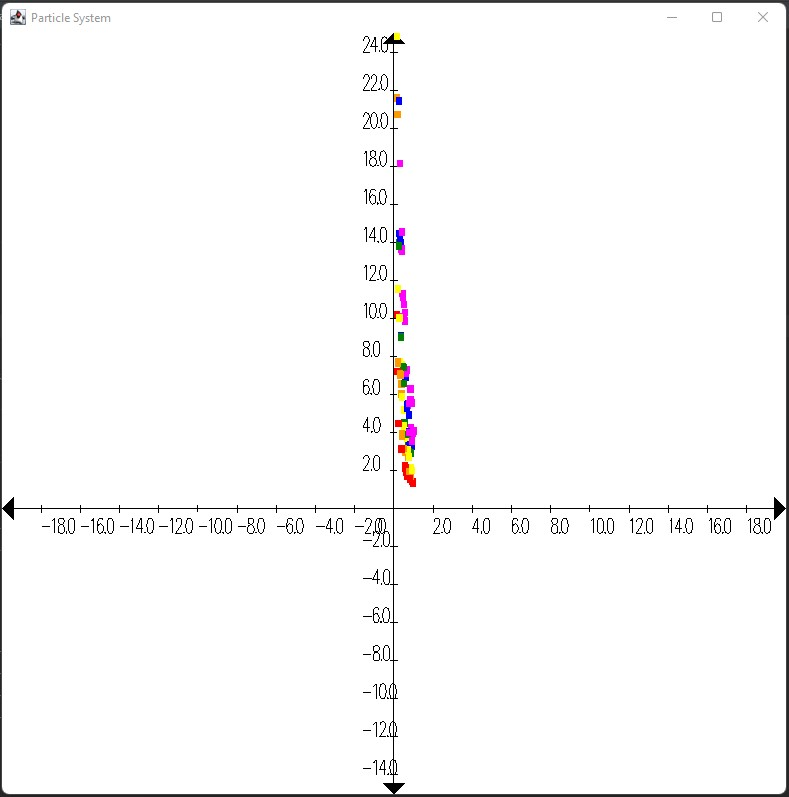
\includegraphics[scale=0.5]{before.jpg}
	\centering
	\caption{Nakon pokretanja algoritma}
	\label{fig:before}
\end{figure}

Kao što se vidi, koordinatni sustav trenutno nije dobro pozicioniran, te su rješenja zbog malog iznosa na x osi, koncentrirana na jedan dio prozora. Taj problem riješila sam mogućnošću translacije i skaliranja koordinatnih osi. Tipkama \textit{strelica gore} i \textit{strelica dolje} pomiče se pogled na koordinatni sustav po y osi, a tipkama \textit{strelica lijevo} i \textit{strelica desno} po x osi. Zatim, tipkama \textit{W} i \textit{S} povećava se odnosno smanjuje skala y osi, a tipkama \textit{A} i \textit{D} skala x osi. Nakon dobre translacije i skaliranja koordinatnog sustava, te nakon par iteracija algoritma, prikaz izgleda kao što prikazuje slika \ref{fig:middle}.
\pagebreak

\begin{figure}[h]
	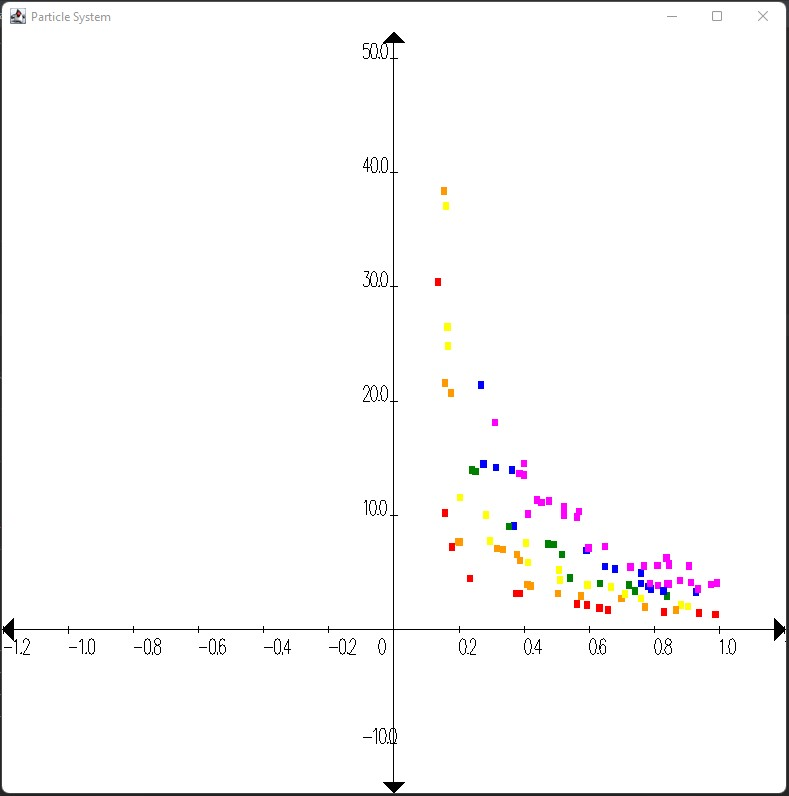
\includegraphics[scale=0.6]{middle.jpg}
	\centering
	\caption{Nakon nekoliko iteracija algoritma}
	\label{fig:middle}
\end{figure}

Može se vidjeti kako su različite fronte prikazane različitim bojama. Najbolja fronta je crvene boje. Zatim fronte idu redoslijedom: narančasta, žuta, zelena, plava, te su sve fronte nakon toga ljubičaste. Par desetaka iteracija kasnije, rješenja se stabiliziraju što se može vidjeti na slici \ref{fig:after}. Sva rješenja su u najboljoj fronti (crvena su), što znači da za svako rješenje ne postoji nijedno drugo koje ga dominira po svim kriterijima.\\
\begin{figure}[h]
	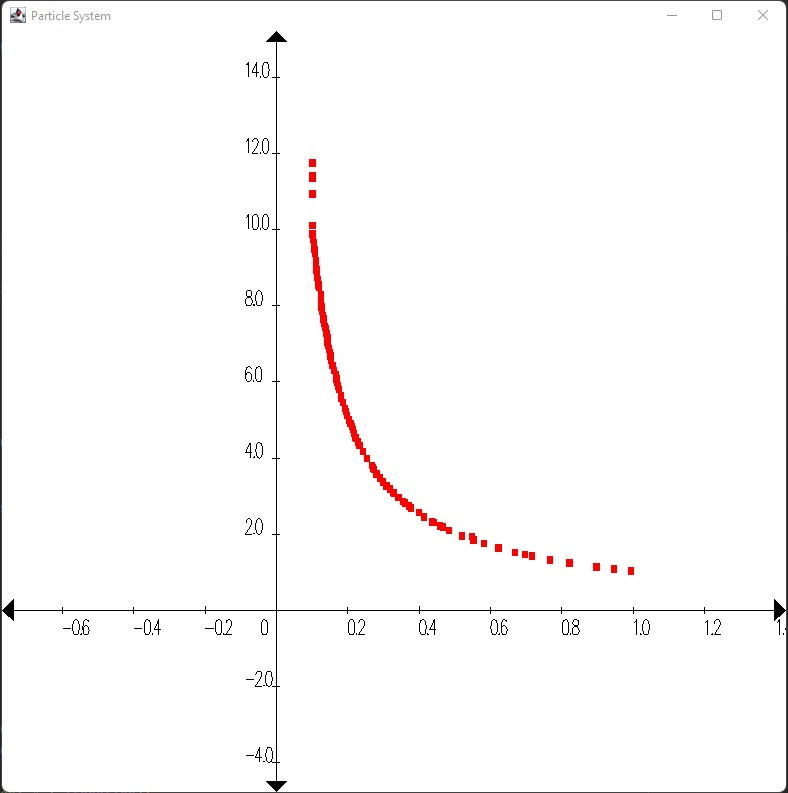
\includegraphics[scale=0.6]{after.jpg}
	\centering
	\caption{Stabilizacija rješenja}
	\label{fig:after}
\end{figure}

Programsko rješenje implementirano je u programskom jeziku Java verzije 11 i koristeći biblioteku OpenGL (odnosno JOGL - Java OpenGL).

\end{document}
